\section{Stable Diffusion}
\label{sec:stable_diffusion}


\begin{figure}
    \centering
    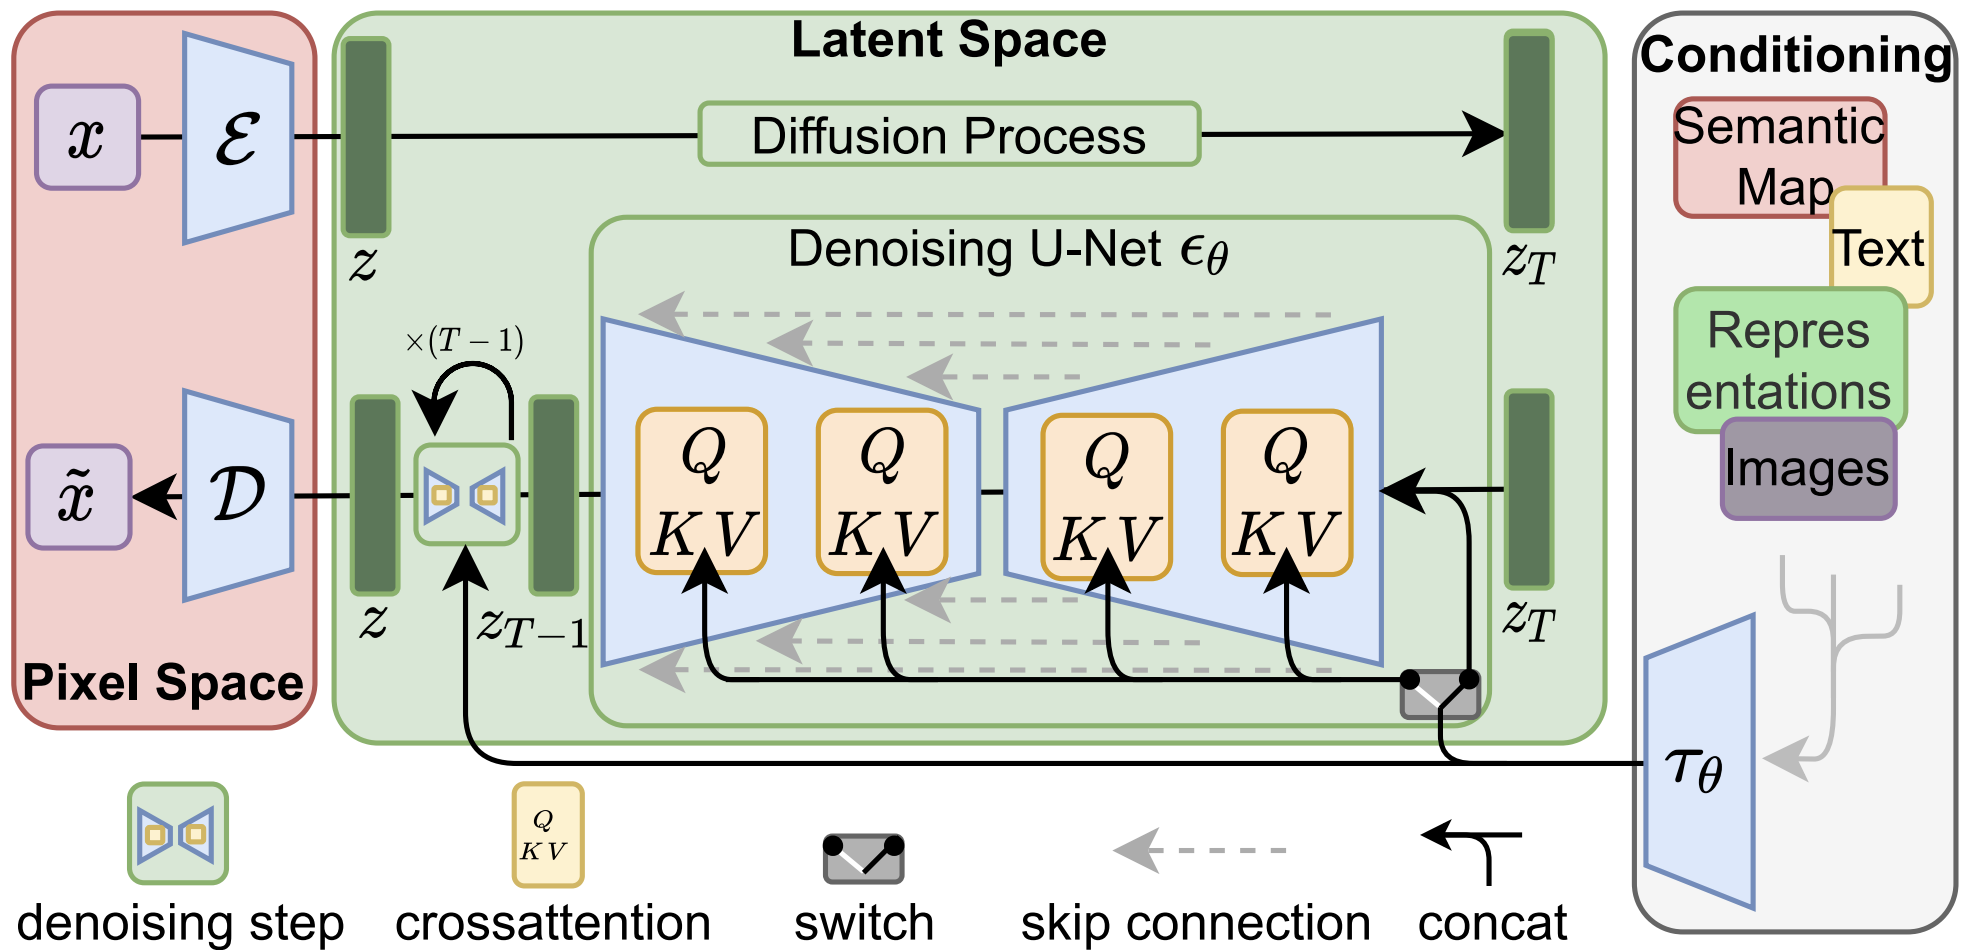
\includegraphics[width=0.8\textwidth]{images/diffusion_models/stable_diffusion/stable_diffusion.png}
    \caption{Stable diffusion scales better compared to other models \cite{stable_diffusion} (DALL-E, VQGAN) with less downsampling blocks (4 instead of 16 as needed by VQGAN).}
\end{figure}


Stable diffusion models are based on latent diffusion. In the paper \cite{stable_diffusion} the authors suggested that computing gradients directly on the pixel space is inefficient, since this space is high-dimentional and includes imperceptible details (high-frequency undesired details). Instead, they suggest to first convert the training images to a lower-dimensional latent space and then apply the diffusion processes on this space. The computation is done on the latent space instead of the pixel space. The authors showed that this approach scales better to higher dimension inputs, and showed significant competitive performance on multiple tasks while lowering significantly computational costs.  And finally, the authors introduced general purpose conditioning mechanism based on cross-attention which allows multi-modal training.

% This process is much more efficient, and in the paper \cite{stable_diffusion} the authors showed that the model can be trained on a single GPU with 16GB of memory. The model is trained on a 256x256 resolution CelebA-HQ dataset with 30 diffusion steps.

% An example of this is when giving an image to a person and asking them to describe the image, they will not describe the individual pixel values, but instead describe the high-level features of the image first.

A 2021 paper released by OpenAI \cite{openai_diffusion_beats_gans} shows that diffusion models can outperform GANs in terms of image fidelity by trading off diversity.














\subsection{U-Net backbone}

U-Net (first introduced in 2015) \cite{unet} is a convolutional neural network architecture that is commonly used in diffusion models, particularly in stable diffusion models and its variants. U-Net is used as a backbone for denoising the latent representations. The U-Net architecture is a symmetric encoder-decoder network with skip connections between the encoder and decoder. The skip connections help the network to learn better, the downsampling process of the encoder removes abstract features in the data, and so skip connections allow the model to skip these downsampling blocks and preserve high-level features. In the original DDPM paper \cite{ddpm} the authors didn't explicitly used U-Net, however they used CNN with residual blocks, which is similar in structure and intent to U-Net. 

\begin{figure}
    \centering
    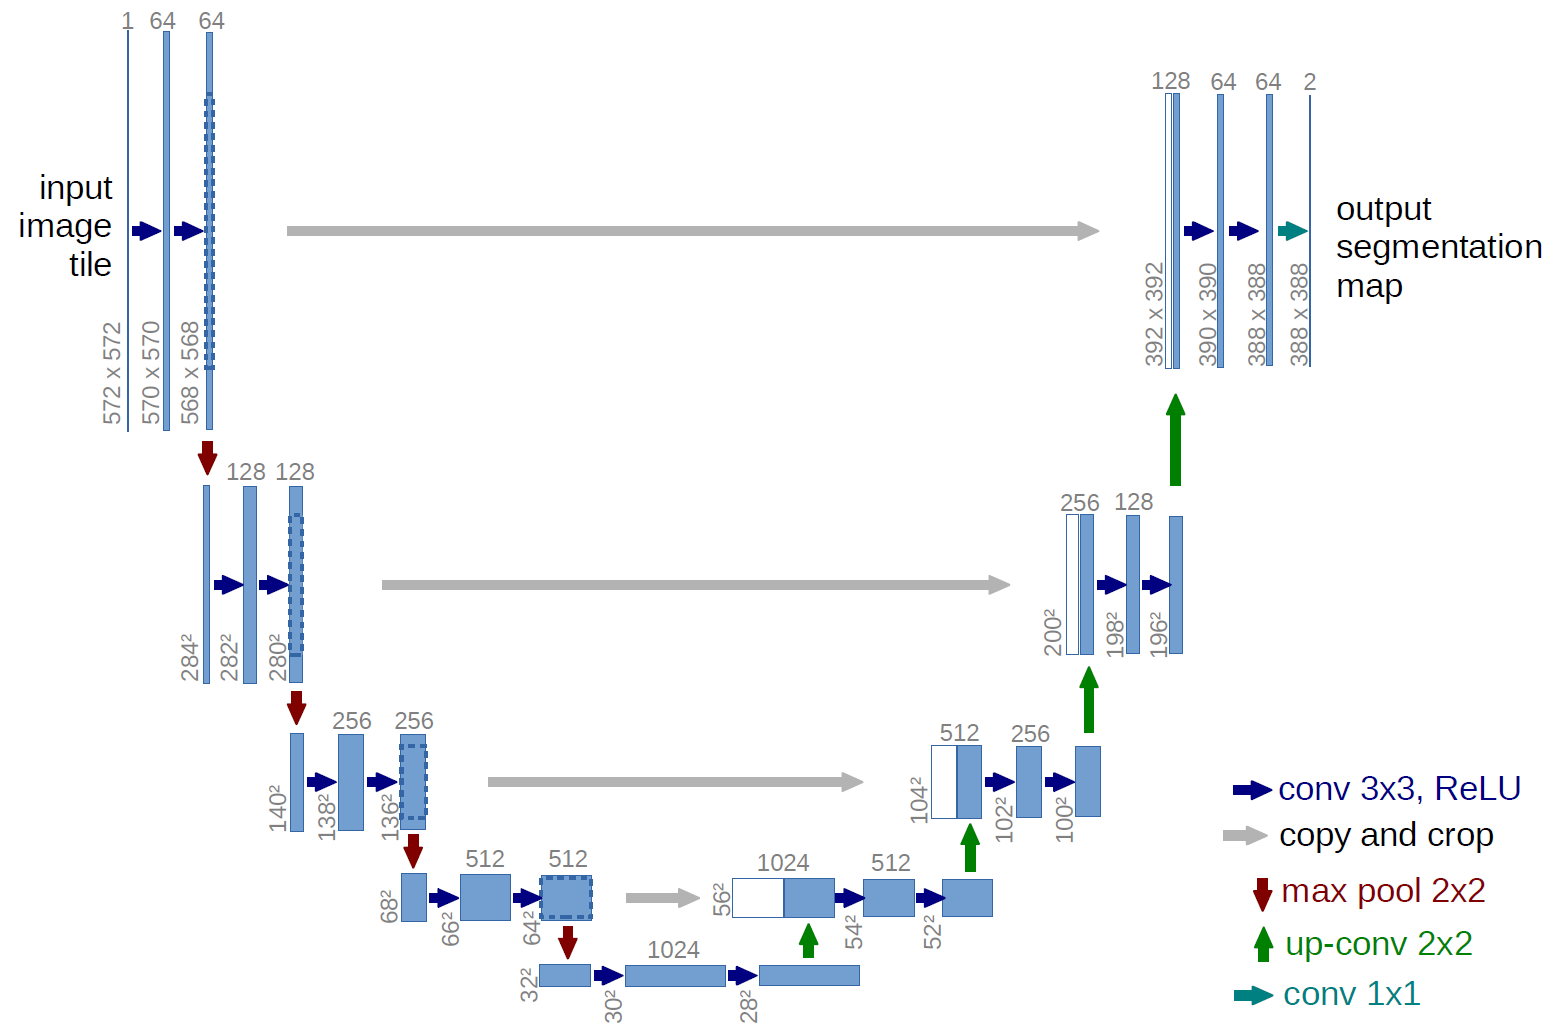
\includegraphics[width=0.8\textwidth]{images/diffusion_models/stable_diffusion/u-net-architecture.png}
    \caption{U-Net architecture \cite{unet}, with convolutional and deconvolutional layers, and skip connections. This architecture is commonly used in stable diffusion models.}
    \label{fig:unet_architecture}
\end{figure}

In figure \ref{fig:unet_architecture} the U-Net is shaped like a 'U' - notice that the layers downsample the input one after the other. Then, after we get to the desired depth, we start upsampling the input until we get output with the same dimensions as the input. The blue arrows are the convolutional layers with kernel size 3x3 and ReLU activation function. The max-pooling are the downsampling layers, and the upsampling layers are the deconvolutional layers.







\subsection{Architecture}

The stable diffusion model, which is a latent diffusion model, consists of: variational autoencoder which compresses the input images into regularized latent space, a U-Net backbone which denoises the output from forward diffusion backwards to obtain a latent representation, a variational autoencoder decoder which converts the latent representation back to the image space, and an optional classifier-free guidance mechanism which allows the model to be conditioned on text prompts or other images, which is domain-specific encoder. The high level architecture is shown in figure \ref{fig:stable_diffusion_architecture}.

\begin{figure}
    \centering
    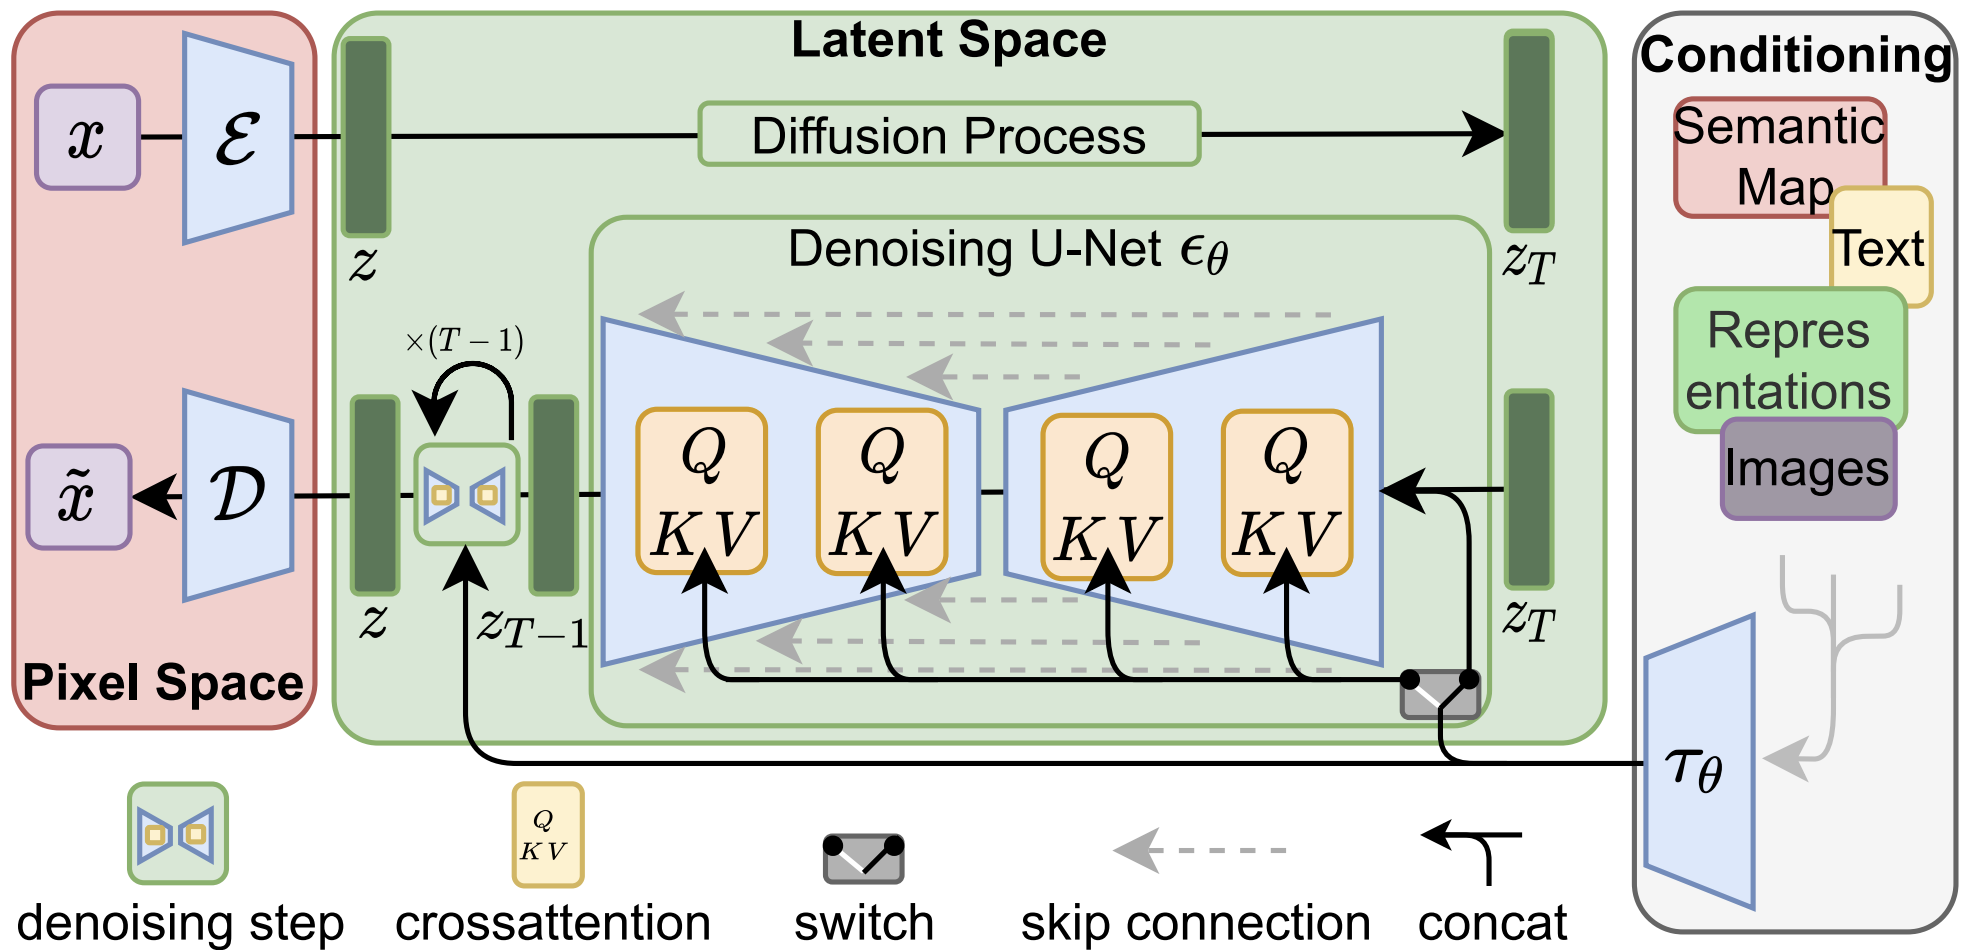
\includegraphics[width=0.75\textwidth]{images/diffusion_models/stable_diffusion/architecture.png}
    \caption{Stable diffusion architecture \cite{stable_diffusion}.}
    \label{fig:stable_diffusion_architecture}
\end{figure}

How the model is able to denoise latent space but also consider the conditional information? The authors used \textbf{cross-attention} mechanism. The cross-attention which was introduced in the transformers paper \cite{transformer}, is a mechanism that allows the model to focus on different parts of the input sequence. In the stable diffusion model, the cross-attention mechanism is used to focus on the latent space and the conditioning signal (text prompt or another image). 








\subsection{Classifier-free diffusion guidance}

\label{subsec:classifier_free_diffusion_guidance}

Conditioning a generative model can be done in many ways. How can we let our model understand our text prompt? Or condition on another image? One way is to train a model to learn a joint distribution of the training data and the conditioning signal $p(x,c)$ and then sample from the joint distribution. This, however, requires the training of a model for each seperate conditioning signal.

Another approach is called \textbf{classifier guidance} \cite{openai_diffusion_beats_gans} which involves the training of a seperate model to condition the output. The latest and most successful approach is called \textbf{classifier-free guidance} \cite{classifier_free_guidance}, in which, instead of training two networks, one conditional network and an unconditional network, we train a single network and during training, with some probability, we set the conditioning signal to zero. This way the network becomes a mix of conditined and unconditioned network, and we can take the conditioned and unconditioned output and combine them with weight that indicates how much we want the network to pay attention to the conditioning signal.








\subsection{Contrastive Language Image Pre-training (CLIP)}

\label{subsec:clip}

CLIP (Contrastive Language Image Pre-training) \cite{openai_clip} is a model that learns visual concepts from text supervision. The CLIP model (which is a pre-trained network) dataset is an image-text pairs (in the paper its 400 million image, text pairs). The model builds associations between images and text prompts. 

\begin{figure}
    \centering
    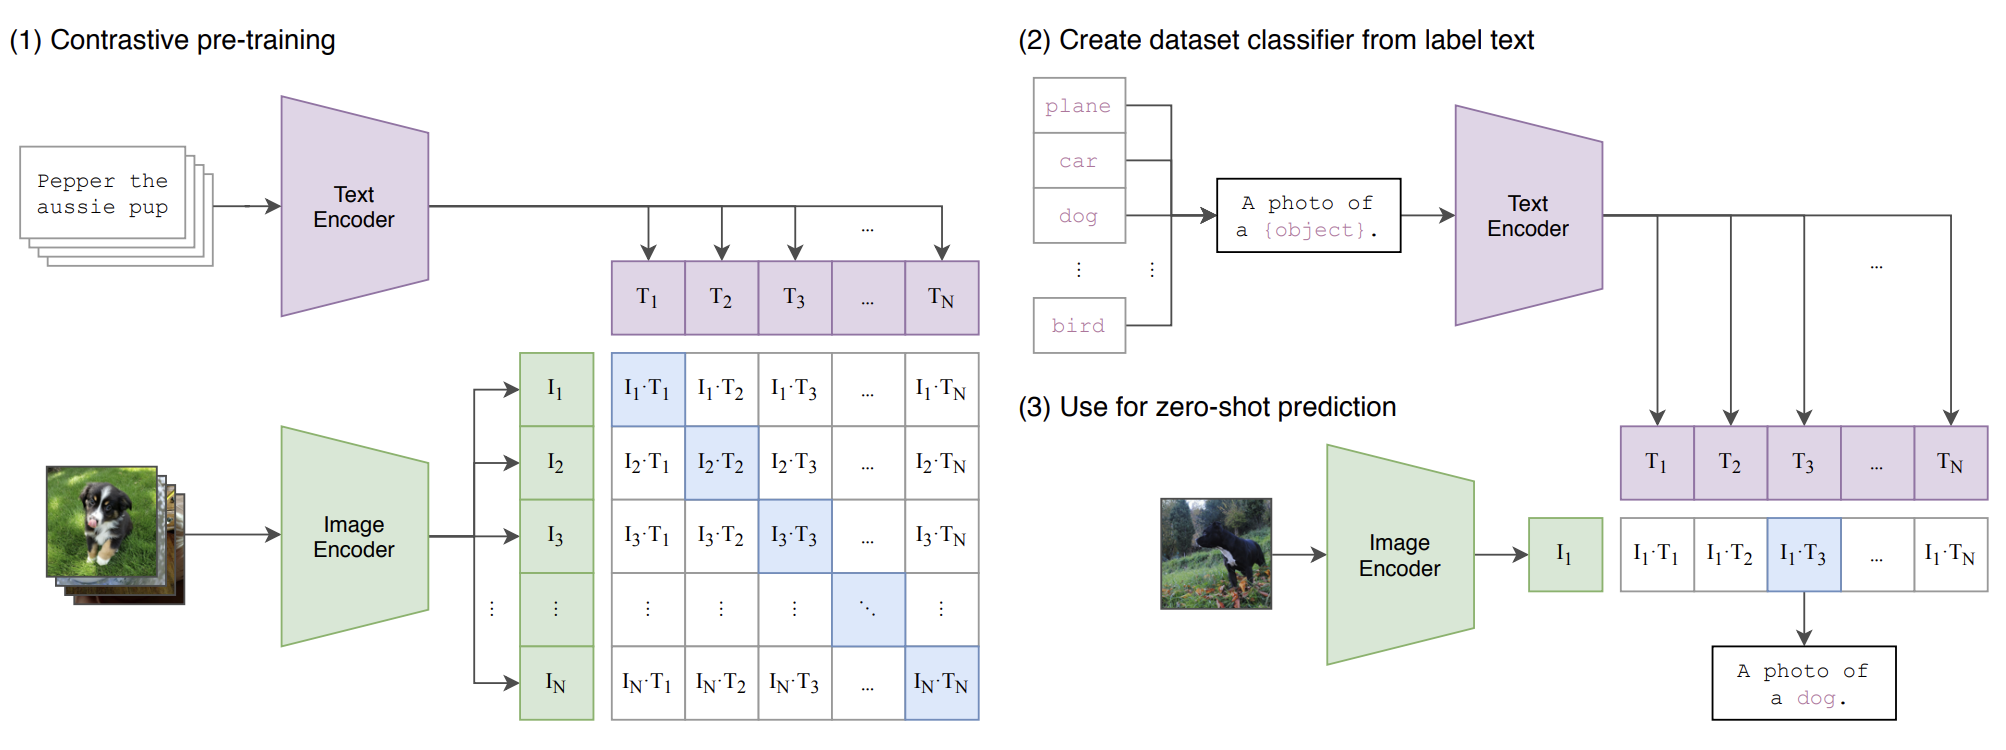
\includegraphics[width=1\textwidth]{images/diffusion_models/stable_diffusion/clip.png}
    \caption{(1) Contrastive pre-training stage of a CLIP model \cite{openai_clip}. The $I_1, ..., I_N$ are the images, and $T_1, ..., T_N$ are the text prompts. The output is a matrix of similarity scores between the images and the text prompts. (2) and (3) after the model is pre-trained its used as a zero-shot image classifier.}
    \label{fig:openai_clip}
\end{figure}

In figure \ref{fig:openai_clip}, intuitively, the main diagonal of the matrix should all be matching '1' (maximum score), and all other cells $\forall i,t \in \{1, ..., N\}, i \neq t, I_i \cdot T_t$ should be '0' (minimal score) since the model learns to associate each prompt with its corresponding image.

The network implementation of CLIP is made up of an image encoder, which is typically a vision transformer \cite{vision_transformer} or a ResNet \cite{resnet} model, while the text encoder is a text transformer \cite{transformer} or continous bag of words \cite{cbow_word2vec} (more commonly known as Word2Vec model by Google, 2013).

In Stable Diffusion, the authors used the text encoder from CLIP. % TODO: Verify, read the paper.












\subsection{Training}

Stable diffusion uses two-stage approach, called classifier-free guidance (see \ref{subsec:classifier_free_diffusion_guidance}) which was discuessed before. In the paper the authors made simplified loss objective:

\[
    L_{\text{DM}} = \mathcal{E}_{x, \epsilon \sim \mathcal{N} (0, 1), t} [ \Vert \epsilon - \epsilon_\theta(x_t, t) \Vert _2^2 ]
\]